\section{Cấu trúc hệ thống và các thành phần}


Hệ thống xem xét gồm các thiết bị người dùng (UE) muốn offload tác vụ lên một máy chủ biên (Edge Server - ES) đặt tại trạm Access Point (AP) gần đó; AP này được hỗ trợ bởi một RIS nhằm cải thiện kênh liên lạc (Hình 1). Giả sử AP có trang bị $M$ ăng-ten thu phát (một trạm nhiều ăng-ten hoặc trạm MIMO), mỗi UE có một ăng-ten, và RIS có $N$ phần tử phản xạ có thể điều chỉnh (với $N$ lớn) \cite{ris_latency}
. Tập các UE được ký hiệu $ \mathcal{U}$, tập các ăng-ten AP ký hiệu $ \mathcal{M}$
. Các UE có thể chia sẻ phổ bằng kỹ thuật ghép kênh phân chia tần số (FDM), nghĩa là mỗi UE được cấp một băng tần con riêng để tránh giao thoa với nhau
. Tổng băng thông hệ thống dành cho đường truyền MEC là $B$ Hz, phân chia cho $K$ UE: mỗi UE $k$ dùng băng thông $B_k$ Hz với $\sum_{k=1}^K B_k = B$ \cite{ris_latency}. 


Hoạt động của MEC diễn ra theo chuỗi thời gian rời rạc: thời gian được chia thành các slot bằng nhau độ dài $T$ (giây) đánh số $t = 1, 2, ...$
. Mỗi slot $T$ được chia thành hai phần: phần điều khiển (overhead điều khiển) và phần payload (dùng để truyền dữ liệu offload)
. Ký hiệu $\tau$ (tau) là tổng thời lượng phần điều khiển trong mỗi slot, khi đó thời gian còn lại cho truyền dữ liệu là $T - \tau$
\cite{ris_latency}
. Thông thường, $T$ được chọn tương ứng với thời gian hiệu dụng kênh (coherence time) sao cho kênh có thể coi là không đổi trong suốt một slot
. Như vậy, nếu kênh thay đổi chậm, ta có thể dùng slot dài để giảm tần suất điều khiển; nếu kênh thay đổi nhanh (ví dụ UE di chuyển tốc độ cao), slot phải ngắn để kịp theo kênh, nhưng chi phí là overhead sẽ chiếm tỷ lệ lớn hơn. 

\begin{figure}[H]
  \centering
  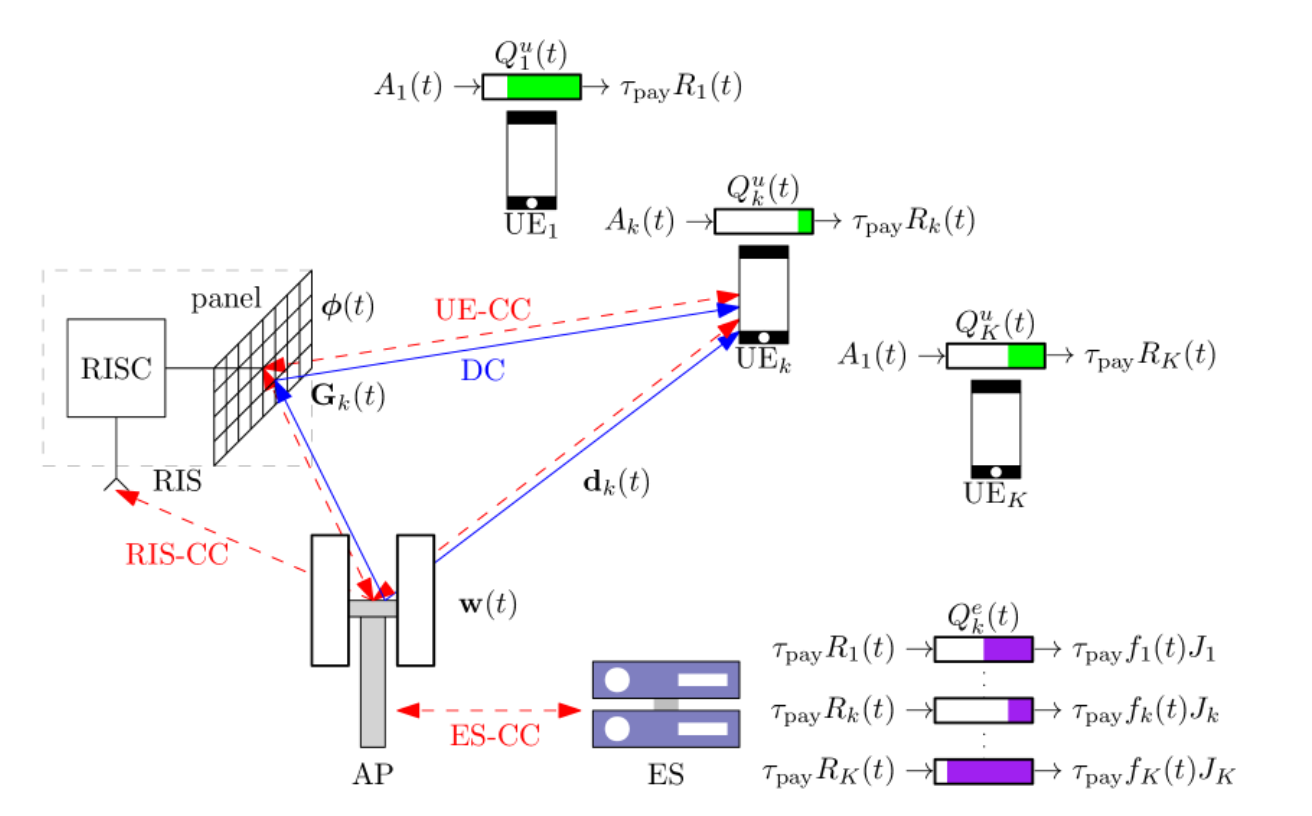
\includegraphics[width=0.8\textwidth]{images/f1.png}
  \caption{Mô hình hệ thống RIS-aided MEC}
    \label{fig:my-image}
\end{figure}



 Máy chủ MEC đặt tại AP chịu trách nhiệm xử lý các tác vụ nhận từ UE. Mỗi UE có một hàng đợi cục bộ để lưu trữ dữ liệu công việc chưa truyền, trong khi ES có một hàng đợi từ xa để lưu các dữ liệu đã nhận chờ xử lý
. Mô hình hàng đợi động: giả sử tại mỗi slot, UE $k$ sinh ra $A_k(t)$ (bit) dữ liệu mới vào hàng đợi cục bộ. Nếu UE truyền được $X_k(t)$ (bit) trong slot đó lên AP thành công, hàng đợi cục bộ sẽ giảm bớt tương ứng. Hàng đợi cục bộ của UE $k$ cập nhật theo công thức: $Q_k^\text{local}(t+1) = \max{Q_k^\text{local}(t) - X_k(t), 0} + A_k(t)$
\cite{ris_latency}
. Tại phía ES, nếu ES xử lý $Y_k(t)$ (bit) cho UE $k$ trong slot (sử dụng tài nguyên CPU), hàng đợi từ xa giảm đi, và đồng thời hàng đợi từ xa tăng thêm chính lượng $X_k(t)$ đã nhận vào. Biểu diễn: $Q_k^\text{ES}(t+1) = \max{Q_k^\text{ES}(t) - Y_k(t), 0} + X_k(t)$
. Độ trễ offload trung bình mà UE $k$ cảm nhận có thể được tính từ hàng đợi tổng (gộp local + ES) theo lý thuyết hàng đợi
, chẳng hạn khi hệ ổn định và $A_k(t)$ ổn định quanh tốc độ trung bình $\lambda_k$ (bit/s), độ trễ trung bình $D_k = \frac{Q_k^\text{local} + Q_k^\text{ES}}{\lambda_k}$
\cite{ris_latency}
.



